\section{Testing}

Testing agent-based models is difficult because the interaction of agents in a
simulation is dynamic and possibly random which produces complex patterns and
behaviours. Traditional software testing strategies which use the divide and
conquer approach can be applied but will typically miss some undesirable
possibilities due the emergent nature of agent-based systems.

Envisioned possibilities can be easily tested but when a model diverges from
its intended path the relationship between variables could show a bug or even
an unexpected solution. The invariants to a simulation, the relationship of
variables that remain true, can be pre-written or detected during simulation
runs and provide a dynamic way of testing agent-based models.

The testing of individual parts of a system is still achieved by unit testing
but testing the interaction of these parts, interation testing, can use
techniques designed for state machines, and the use of invarient detectors.

\subsection{Unit Testing}

Unit testing is the testing of individual modules of a piece of software, in the
case of models these are the individual agent functions. Each function has an
accompanying unit test function that sets the initial agent memory and any input,
calls the function, and assets that the new agent memory and outputs are what
was expected.

FLAME provides procedures to help with unit testing:

\begin{itemize}
  \item initialise\_unit\_testing() -- initialises FLAME for unit testing agent
  functions, required at the start of a testing suite.
  \item unittest\_init\_agentname\_agent() -- initialises the agent memory that
  will used in testing
  \item The agent memory is then updated
  \item Messages are sent that will be the input to the function to be tested
  \item The function to be tested is called
  \item Assertions are tested against the resulting agent memory and any output
  \item unittest\_free\_agentname\_agent() -- the agent memory is deleted
  \item free\_messages() -- any messages used are deleted
  \item clean\_up() -- FLAME is finalised and ready to end.
\end{itemize}

\begin{figure}[hb]
\centering
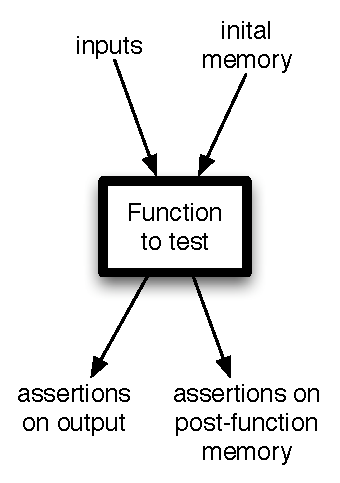
\includegraphics[scale=1.0]{unittest.eps}
\caption{Unit testing}
\label{fig:unittesting}
\end{figure}

\subsection{Integration Testing}

The testing of combinations of program modules up to the level of the whole
system.

Need coverage of testing combinations, a test set.

The W-method proposed by T. Chow \cite{CHOW:1978} provides a complete test set
of sequences through a state machine.

Used an implementation called statechum (http://statechum.sourceforge.net/)
that accepts graphml as input. Converted each agent into a separate state
machine as graphml. 

One way to analyse the output of runs is to use an invarient detector. This
program reports any likely invariants, properties that hold at certain points.
This could then be analysed by the modeller and possibly used as assertions in
future test runs.

The Daikon invariant detector (http://groups.csail.mit.edu/pag/daikon/)
\cite{DAIKON:2007}.

{\tiny
\begin{verbatim}
#1 [Firm_idle, Firm_receive_data, Firm_calc_production_quantity]
#2 [Firm_idle, Firm_idle, Firm_calc_production_quantity, Firm_calc_input_demands, 
    Firm_compute_total_liquidity_needs, Firm_idle, Firm_execute_financial_payments, 
    Firm_calculate_specific_skills_and_wage_offer, Firm_idle, Firm_read_job_quitting,
    Firm_finish_labour_market_first_round, Firm_read_job_quitting_2, Firm_idle,
    Firm_compute_mean_wage_specific_skills, Firm_send_capital_demand,
    Firm_receive_capital_goods, Firm_execute_production, Firm_calc_pay_costs,
    Firm_send_goods_to_mall, Firm_calc_revenue]
#3 [Firm_idle, Firm_idle, Firm_calc_production_quantity, Firm_calc_input_demands,
    Firm_compute_total_liquidity_needs, Firm_idle, Firm_execute_financial_payments,
    Firm_calculate_specific_skills_and_wage_offer, Firm_idle, Firm_read_job_quitting,
    Firm_finish_labour_market_first_round, Firm_read_job_quitting_2,
    Firm_update_wage_offer_2, Firm_compute_mean_wage_specific_skills]
#4 [Firm_idle, Firm_idle, Firm_calc_production_quantity, Firm_calc_input_demands,
    Firm_compute_total_liquidity_needs, Firm_idle, Firm_execute_financial_payments,
    Firm_calculate_specific_skills_and_wage_offer, Firm_idle, Firm_read_job_quitting,
    Firm_start_labour_market, Firm_send_vacancies_2,
    Firm_read_job_applications_send_job_offer_or_rejection_2, Firm_read_job_responses_2,
    Firm_read_job_quitting_2, Firm_idle]
#5 [Firm_idle, Firm_idle, Firm_calc_production_quantity, Firm_calc_input_demands,
    Firm_compute_total_liquidity_needs, Firm_idle, Firm_execute_financial_payments,
    Firm_calculate_specific_skills_and_wage_offer, Firm_send_vacancies,
    Firm_read_job_applications_send_job_offer_or_rejection, Firm_read_job_responses,
    Firm_read_job_quitting, Firm_finish_labour_market_first_round, Firm_read_job_quitting_2,
    Firm_idle]
#6 [Firm_idle, Firm_idle, Firm_calc_production_quantity, Firm_calc_input_demands,
    Firm_compute_total_liquidity_needs, Firm_idle, Firm_execute_financial_payments,
    Firm_calculate_specific_skills_and_wage_offer, Firm_send_vacancies,
    Firm_read_job_applications_send_job_offer_or_rejection, Firm_read_job_responses,
    Firm_read_job_quitting, Firm_update_wage_offer, Firm_send_vacancies_2]
#7 [Firm_idle, Firm_idle, Firm_calc_production_quantity, Firm_calc_input_demands,
    Firm_compute_total_liquidity_needs, Firm_apply_for_loans, Firm_read_loan_acceptance,
    Firm_idle, Firm_execute_financial_payments]
#8 [Firm_idle, Firm_idle, Firm_calc_production_quantity, Firm_calc_input_demands,
    Firm_compute_total_liquidity_needs, Firm_apply_for_loans, Firm_read_loan_acceptance,
    Firm_calc_production_quantity_2, Firm_execute_financial_payments]
#9 [Firm_idle, Firm_idle, Firm_set_quantities_zero, Firm_read_job_quitting,
    Firm_read_job_quitting_2, Firm_calc_revenue, Firm_idle, Firm_send_data_to_Eurostat,
    Firm_send_payments_to_bank]
#10 [Firm_idle, Firm_idle, Firm_set_quantities_zero, Firm_read_job_quitting,
     Firm_read_job_quitting_2, Firm_calc_revenue, Firm_compute_sales_statistics,
     Firm_compute_financial_payments, Firm_compute_income_statement, Firm_compute_dividends,
     Firm_compute_total_financial_payments, Firm_compute_balance_sheet,
     Firm_update_specific_skills_of_workers, Firm_idle]
#11 [Firm_idle, Firm_idle, Firm_set_quantities_zero, Firm_read_job_quitting,
     Firm_read_job_quitting_2, Firm_calc_revenue, Firm_compute_sales_statistics,
     Firm_compute_financial_payments, Firm_compute_income_statement, Firm_compute_dividends,
     Firm_compute_total_financial_payments, Firm_compute_balance_sheet, 
     Firm_update_specific_skills_of_workers, Firm_send_data_to_Eurostat]
#12 [Firm_read_tax_rates, Firm_receive_data]
#13 [Firm_read_tax_rates, Firm_idle]
\end{verbatim}
}
